\documentclass[aspectratio=169]{beamer}
\usetheme{Madrid}
\usecolortheme{default}

\usepackage{booktabs}
\usepackage{multirow}
\usepackage{xcolor}
\usepackage{colortbl}
\usepackage{amsmath}
\usepackage{amssymb}
\usepackage{graphicx}
\usepackage{tikz}
\usetikzlibrary{arrows.meta, positioning, shapes, fit, calc}
\usepackage{url}
\usepackage{pifont}
\usepackage{svg}
\usepackage{adjustbox}

% Custom colors
\definecolor{paperblue}{RGB}{51, 102, 153}
\definecolor{reprogreen}{RGB}{34, 139, 34}
\definecolor{warnred}{RGB}{178, 34, 34}
\definecolor{lightgray}{RGB}{240, 240, 240}
\definecolor{elecyellow}{RGB}{255, 193, 7}
\definecolor{causalblue}{RGB}{66, 133, 244}
\definecolor{regimeorange}{RGB}{255, 152, 0}

\setbeamercolor{title}{fg=paperblue}
\setbeamercolor{frametitle}{fg=paperblue}

\title{CaRS: Causal Regime-Switching State Space Model\\for Electricity Price Forecasting}
\subtitle{Combining Deep State Space Models with Causal Structure Learning}
\date{January 2026}

\begin{document}

\begin{frame}
\titlepage
\end{frame}

%==============================================================================
\begin{frame}{Overview}
\tableofcontents
\end{frame}

%==============================================================================
\section{Motivation}

\begin{frame}{Why Electricity Price Estimation \& Prediction?}
\begin{columns}
\begin{column}{0.5\textwidth}
\textbf{Estimation Task:}
\begin{itemize}
    \item Given: $X_{0:t}, Y_{0:t-1}$
    \item Estimate: $Y_t$ (today's price)
    \item \textbf{Use case:} Real-time market analysis, missing data imputation
\end{itemize}

\vspace{0.3cm}
\textbf{Prediction Task:}
\begin{itemize}
    \item Given: $X_{0:t}, Y_{0:t}$
    \item Predict: $Y_{t+1}$ (tomorrow's price)
    \item \textbf{Use case:} Trading decisions, risk management
\end{itemize}
\end{column}

\begin{column}{0.5\textwidth}
\textbf{Why Switching Regimes?}
\begin{itemize}
    \item Energy markets exhibit \textbf{structural breaks}
    \item Different price dynamics during:
    \begin{itemize}
        \item Peak vs. off-peak hours
        \item Summer vs. winter
        \item Normal vs. crisis periods
    \end{itemize}
    \item \textbf{Causal relationships change} across regimes
    \item Single-regime models miss important dynamics
\end{itemize}
\end{column}
\end{columns}

\vspace{0.3cm}
\begin{center}
\fcolorbox{causalblue}{lightgray}{\parbox{0.8\textwidth}{\centering
\textbf{Goal:} Learn regime-specific causal structures that explain\\
\textit{which factors drive prices} and \textit{how this changes over time}
}}
\end{center}
\end{frame}

%------------------------------------------------------------------------------
\begin{frame}{Economic Importance of Electricity Price Modeling}
\begin{columns}
\begin{column}{0.5\textwidth}
\textbf{Energy Security \& Grid Stability}
\begin{itemize}
    \item Accurate price forecasts essential for \textbf{grid balancing}
    \item Misaligned supply/demand $\rightarrow$ blackouts or price spikes
    \item Renewable integration requires understanding price volatility
\end{itemize}

\vspace{0.3cm}
\textbf{Market Efficiency \& Price Discovery}
\begin{itemize}
    \item Transparent pricing mechanisms
    \item Efficient allocation of generation resources
    \item Cross-border trading optimization (DE-FR interconnection)
\end{itemize}
\end{column}

\begin{column}{0.5\textwidth}
\textbf{Financial Risk Management}
\begin{itemize}
    \item Utilities hedge against price volatility
    \item Trading firms require reliable forecasts
    \item Investment decisions for new generation capacity
\end{itemize}

\vspace{0.3cm}
\textbf{Policy \& Consumer Protection}
\begin{itemize}
    \item Carbon pricing impact assessment
    \item Renewable subsidy effectiveness
    \item Consumer electricity bill forecasting
    \item Regulatory compliance (REMIT, EU energy law)
\end{itemize}
\end{column}
\end{columns}
\end{frame}

\begin{frame}{Economic Importance of Electricity Price Modeling}
\begin{center}
\fcolorbox{reprogreen}{lightgray}{\parbox{0.8\textwidth}{\centering
\textbf{Impact:} Understanding \textit{causal} price drivers enables better policy decisions,\\
more efficient markets, and reduced consumer costs.
}}
\end{center}
\end{frame}

%==============================================================================
\section{Technical Challenges}

\begin{frame}{Technical Challenges in Energy Price Modeling}
\begin{columns}
\begin{column}{0.5\textwidth}
\textbf{1. Latent/Unobserved Variables}
\begin{itemize}
    \item Market regimes are \textbf{not directly observable}
    \item Must infer regime from price behavior
    \item Regime transitions follow \textbf{Markov dynamics}
\end{itemize}

\vspace{0.3cm}
\textbf{2. Non-Stationary Transition Dynamics}
\begin{itemize}
    \item Regime transition probabilities change
    \item $P(d_t | d_{t-1})$ varies with market conditions
    \item Standard HMMs assume fixed transitions
\end{itemize}
\end{column}

\begin{column}{0.5\textwidth}
\textbf{3. High-Frequency Data}
\begin{itemize}
    \item Hourly electricity prices
    \item Strong \textbf{autocorrelation} structures
    \item Intraday and weekly seasonality
\end{itemize}

\vspace{0.3cm}
\textbf{4. Non-Linear Dependencies}
\begin{itemize}
    \item Complex interactions between:
    \begin{itemize}
        \item Renewable generation (wind, solar)
        \item Commodity prices (gas, coal, carbon)
        \item Load/demand patterns
    \end{itemize}
    \item Linear models insufficient
\end{itemize}
\end{column}
\end{columns}

\vspace{0.3cm}
\begin{center}
\textcolor{warnred}{\textbf{Challenge:}} How to jointly learn (1) latent regimes, (2) regime-specific causal graphs, and (3) non-linear dynamics?
\end{center}
\end{frame}

%------------------------------------------------------------------------------
\begin{frame}{Beyond Energy Markets: A Generalizable Framework}
\textbf{CaRS addresses common challenges across multiple domains:}

\vspace{0.3cm}
\begin{columns}
\begin{column}{0.5\textwidth}
\textbf{Financial Markets}
\begin{itemize}
    \item Regime shifts: bull/bear markets, volatility clusters
    \item Non-stationary dependencies between assets
    \item Causal drivers change during crises
\end{itemize}

\vspace{0.2cm}
\textbf{Healthcare \& Epidemiology}
\begin{itemize}
    \item Patient monitoring with changing conditions
    \item Disease progression with treatment regimes
    \item Epidemic dynamics (normal vs. outbreak)
\end{itemize}
\end{column}

\begin{column}{0.5\textwidth}
\textbf{Climate Science}
\begin{itemize}
    \item Weather pattern regime shifts (El Ni\~{n}o/La Ni\~{n}a)
    \item Non-linear climate feedback mechanisms
    \item Changing causal relationships over seasons
\end{itemize}

\vspace{0.2cm}
\textbf{Manufacturing \& IoT}
\begin{itemize}
    \item Process monitoring with multiple operating modes
    \item Quality control under varying conditions
    \item Predictive maintenance with regime detection
\end{itemize}
\end{column}
\end{columns}

\vspace{0.3cm}
\begin{center}
\fcolorbox{causalblue}{lightgray}{\parbox{0.85\textwidth}{\centering
\textbf{Key Insight:} Any domain with (1) latent regimes, (2) changing causal structures, and (3) non-linear dynamics can benefit from CaRS.
}}
\end{center}
\end{frame}

%==============================================================================
\section{Literature Review}

\begin{frame}{Model Comparison: Capabilities}
\begin{table}
\centering
\small
\begin{tabular}{l|ccccc}
\toprule
\textbf{Model} & \textbf{Regime} & \textbf{Causal} & \textbf{Temporal} & \textbf{Non-Linear} & \textbf{Interpretable} \\
& \textbf{Switching} & \textbf{DAGs} & \textbf{Dynamics} & \textbf{Relations} & \textbf{Graphs} \\
\midrule
ARIMA/VAR & \textcolor{warnred}{\ding{55}} & \textcolor{warnred}{\ding{55}} & \textcolor{reprogreen}{\ding{51}} & \textcolor{warnred}{\ding{55}} & \textcolor{warnred}{\ding{55}} \\
MS-VAR & \textcolor{reprogreen}{\ding{51}} & \textcolor{warnred}{\ding{55}} & \textcolor{reprogreen}{\ding{51}} & \textcolor{warnred}{\ding{55}} & \textcolor{warnred}{\ding{55}} \\
NOTEARS/GOLEM & \textcolor{warnred}{\ding{55}} & \textcolor{reprogreen}{\ding{51}} & \textcolor{warnred}{\ding{55}} & \textcolor{reprogreen}{\ding{51}} & \textcolor{reprogreen}{\ding{51}} \\
DYNOTEARS & \textcolor{warnred}{\ding{55}} & \textcolor{reprogreen}{\ding{51}} & \textcolor{reprogreen}{\ding{51}} & \textcolor{warnred}{\ding{55}} & \textcolor{reprogreen}{\ding{51}} \\
DS3M & \textcolor{reprogreen}{\ding{51}} & \textcolor{warnred}{\ding{55}} & \textcolor{reprogreen}{\ding{51}} & \textcolor{reprogreen}{\ding{51}} & \textcolor{warnred}{\ding{55}} \\
FANTOM & \textcolor{reprogreen}{\ding{51}} & \textcolor{reprogreen}{\ding{51}} & \textcolor{reprogreen}{\ding{51}} & \textcolor{reprogreen}{\ding{51}} & \textcolor{reprogreen}{\ding{51}} \\
\midrule
\textbf{CaRS} & \textcolor{reprogreen}{\ding{51}} & \textcolor{reprogreen}{\ding{51}} & \textcolor{reprogreen}{\ding{51}} & \textcolor{reprogreen}{\ding{51}} & \textcolor{reprogreen}{\ding{51}} \\
\bottomrule
\end{tabular}
\end{table}

\vspace{0.3cm}
\textbf{Key References:}
\begin{itemize}
    \item \textbf{DS3M} (Xu et al., 2021): Deep Switching State Space Model for time series
    \item \textbf{FANTOM} (Rahmani et al., 2025): Causal discovery with regime switching
    \item \textbf{NOTEARS} (Zheng et al., 2018): Differentiable DAG learning
\end{itemize}
\end{frame}

%==============================================================================
\section{Economic Relevance}

\begin{frame}{Why Causal Models for Decision Making?}
\begin{columns}
\begin{column}{0.33\textwidth}
\textbf{Interpretability}
\begin{itemize}
    \item Understand \textit{why} prices change
    \item Identify key drivers per regime
    \item Communicate to stakeholders
    \item Regulatory compliance
\end{itemize}
\end{column}

\begin{column}{0.33\textwidth}
\textbf{Trustworthiness}
\begin{itemize}
    \item Causal graphs can be validated by domain experts
    \item Predictions grounded in economic theory
    \item Detect spurious correlations
    \item Build confidence in model outputs
\end{itemize}
\end{column}

\begin{column}{0.33\textwidth}
\textbf{Robustness}
\begin{itemize}
    \item Causal models generalize better under \textbf{distribution shift}
    \item Regime-specific DAGs adapt to changing conditions
    \item More stable predictions during market stress
\end{itemize}
\end{column}
\end{columns}
\end{frame}

\begin{frame}{Why Causal Models for Decision Making?}
\begin{center}
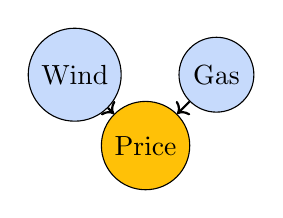
\begin{tikzpicture}[scale=0.6]
\node[draw, circle, fill=elecyellow] (price) at (0,0) {Price};
\node[draw, circle, fill=causalblue!30] (wind) at (-1.5,1.5) {Wind};
\node[draw, circle, fill=causalblue!30] (gas) at (1.5,1.5) {Gas};
\draw[->, thick] (wind) -- (price);
\draw[->, thick] (gas) -- (price);
\end{tikzpicture}
\end{center}
\begin{center}
\fcolorbox{reprogreen}{lightgray}{\parbox{0.9\textwidth}{\centering
\textbf{Benefit for Energy Trading:} Knowing that ``wind generation $\rightarrow$ price'' is causal (not just correlated) enables better hedging strategies and scenario analysis under different weather conditions.
}}
\end{center}
\end{frame}

%==============================================================================
\section{Data}

\begin{frame}{Data Description: European Electricity Markets}
\begin{columns}
\begin{column}{0.5\textwidth}
\textbf{Target Variables:}
\begin{itemize}
    \item \textbf{DE}: German day-ahead price (EUR/MWh)
    \item \textbf{FR}: French day-ahead price (EUR/MWh)
    \item \textbf{DE\_FR}: Spread modeling
\end{itemize}

\vspace{0.3cm}
\textbf{Explanatory Features (18 total):}
\begin{itemize}
    \item \textbf{Generation}: Wind, Solar, Hydro, Nuclear, Gas, Coal
    \item \textbf{Demand}: Residual Load
    \item \textbf{Commodities}: Natural Gas, Brent Oil, WTI Oil
    \item \textbf{Weather}: Temperature, Rain
    \item \textbf{Temporal}: Hour, Day of week
\end{itemize}
\end{column}

\begin{column}{0.5\textwidth}
\textbf{Data Statistics:}
\begin{table}
\scriptsize
\begin{tabular}{l|cc}
\toprule
& \textbf{DE} & \textbf{FR} \\
\midrule
Period & 2015-2024 & 2015-2024 \\
Frequency & Daily & Daily \\
Train windows & 2,537 & 2,537 \\
Test windows & 694 & 694 \\
Mean price & 89.5 EUR & 102.3 EUR \\
Std dev & 145.2 EUR & 168.7 EUR \\
Min & -130 EUR & -75 EUR \\
Max & 870 EUR & 3,000 EUR \\
\bottomrule
\end{tabular}
\end{table}

\vspace{0.2cm}
\textbf{Key characteristics:}
\begin{itemize}
    \item Heavy tails, negative prices
    \item Strong autocorrelation
    \item Regime changes (energy crisis 2022)
\end{itemize}
\end{column}
\end{columns}
\end{frame}

%------------------------------------------------------------------------------
\begin{frame}{Time Series: Germany Day-Ahead Prices (2015-2024)}
\begin{center}
\includesvg[height=0.85\textheight]{figures/de_unified_timeseries.svg}
\end{center}
\end{frame}

%------------------------------------------------------------------------------
\begin{frame}{Time Series: France Day-Ahead Prices (2015-2024)}
\begin{center}
\includesvg[height=0.85\textheight]{figures/fr_unified_timeseries.svg}
\end{center}
\end{frame}

%==============================================================================
\section{Methodology}

\begin{frame}{Model Overview: CaRS}
\begin{columns}
\begin{column}{0.5\textwidth}
\textbf{DS3M\_UV (Univariate)}
\begin{itemize}
    \item Only uses target $Y$
    \item Autoregressive regime switching
    \item Strong baseline for price forecasting
\end{itemize}

\vspace{0.3cm}
\textbf{DS3M\_MV (Multivariate)}
\begin{itemize}
    \item Uses features $X$ and target $Y$
    \item Black-box emission network
    \item No interpretable structure
\end{itemize}
\end{column}

\begin{column}{0.5\textwidth}
\textbf{CaRS (Ours)}
\begin{itemize}
    \item Combines SSM regime switching with causal discovery
    \item \textbf{Key innovation:} Enhances SSM with Invertible Contractive Graph Neural Network (ICGNN)%Replace DS3M's emission network with FANTOM's ICGNN
    \item Learns \textbf{sparse causal DAGs per regime}
\end{itemize}

% \vspace{0.1cm}
\textbf{FANTOM\_BEM (Baseline)}
\begin{itemize}
    \item Bayesian EM for regime detection
    \item Full FANTOM causal discovery
    \item Reference implementation
\end{itemize}
\end{column}
\end{columns}

% \vspace{0.3cm}
\begin{center}
\fcolorbox{causalblue}{lightgray}{\parbox{0.9\textwidth}{\centering
\textbf{Novelty:} CaRS merges deep state-space temporal modeling (DS3M) with differentiable causal graph learning (FANTOM), enabling \textit{interpretable regime-specific predictions}.
}}
\end{center}
\end{frame}

%------------------------------------------------------------------------------
\begin{frame}{Key Methodological Differences: DS3M vs FANTOM vs CaRS}
\begin{table}
\centering
\small
\begin{tabular}{l|ccc}
\toprule
\textbf{Component} & \textbf{DS3M} & \textbf{FANTOM} & \textbf{CaRS (Ours)} \\
\midrule
\textbf{Temporal Encoding} & GRU & None & GRU \\
\textbf{Regime Detection} & Markov (learnable) & Bayesian EM & Markov (learnable) \\
\textbf{State Space} & Continuous $z_t$ & None & Continuous $z_t$ \\
\textbf{Emission Model} & Black-box MLP & ICGNN & ICGNN \\
\textbf{Causal Graphs} & \textcolor{warnred}{None} & Per-regime DAGs & Per-regime DAGs \\
\textbf{DAG Learning} & -- & Gumbel-Softmax & Gumbel-Softmax \\
\textbf{Noise Modeling} & Gaussian & Cond. Norm. Flows & Gaussian \\
\bottomrule
\end{tabular}
\end{table}

% \vspace{0.1cm}
\textbf{What each method contributes:}
\begin{columns}
\begin{column}{0.33\textwidth}
\textcolor{paperblue}{\textbf{From DS3M:}}
\begin{itemize}
    \item GRU temporal encoding
    \item Learnable Markov regimes
    \item Continuous latent state
\end{itemize}
\end{column}

\begin{column}{0.33\textwidth}
\textcolor{paperblue}{\textbf{From FANTOM:}}
\begin{itemize}
    \item ICGNN architecture
    \item Differentiable DAG learning
    \item Sparsity constraints
\end{itemize}
\end{column}

\begin{column}{0.33\textwidth}
\textcolor{reprogreen}{\textbf{CaRS Innovation:}}
\begin{itemize}
    \item Unified framework
    \item Interpretable + temporal
    \item Scalable training
\end{itemize}
\end{column}
\end{columns}
\end{frame}

%==============================================================================
\begin{frame}{CaRS: Architecture}
\begin{center}
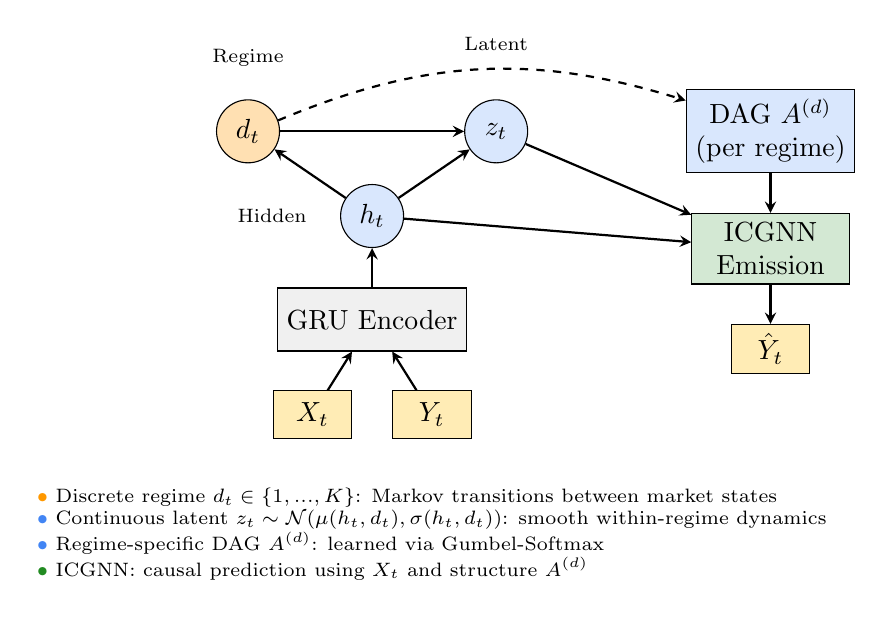
\begin{tikzpicture}[
    node distance=1.2cm,
    block/.style={draw, rectangle, minimum width=2cm, minimum height=0.8cm, align=center},
    latent/.style={draw, circle, minimum size=0.8cm, fill=causalblue!20},
    observed/.style={draw, rectangle, minimum width=1cm, minimum height=0.6cm, fill=elecyellow!30},
    arrow/.style={->, thick, >=stealth}
]

% Input
\node[observed] (x) {$X_t$};
\node[observed, right=0.5cm of x] (y) {$Y_t$};

% GRU Encoder
\node[block, above=0.8cm of $(x)!0.5!(y)$, fill=lightgray] (gru) {GRU Encoder};
\draw[arrow] (x) -- (gru);
\draw[arrow] (y) -- (gru);

% Hidden state
\node[latent, above=0.5cm of gru] (h) {$h_t$};
\node[left=0.3cm of h, font=\scriptsize] {Hidden};
\draw[arrow] (gru) -- (h);

% Discrete regime
\node[latent, above left=0.5cm and 1cm of h, fill=regimeorange!30] (d) {$d_t$};
\node[above=0.3cm of d, font=\scriptsize] {Regime};
\draw[arrow] (h) -- (d);

% Continuous latent
\node[latent, above right=0.5cm and 1cm of h] (z) {$z_t$};
\node[above=0.5cm of z, font=\scriptsize] {Latent};
\draw[arrow] (h) -- (z);
\draw[arrow] (d) -- (z);

% DAG per regime
\node[block, right=2cm of z, fill=causalblue!20] (dag) {DAG $A^{(d)}$\\(per regime)};
\draw[arrow, dashed] (d) to[bend left=20] (dag);

% ICGNN
\node[block, below=0.5cm of dag, fill=reprogreen!20] (icgnn) {ICGNN\\Emission};
\draw[arrow] (dag) -- (icgnn);
\draw[arrow] (z) -- (icgnn);
\draw[arrow] (h) -- (icgnn);

% Output
\node[observed, below=0.5cm of icgnn] (yhat) {$\hat{Y}_t$};
\draw[arrow] (icgnn) -- (yhat);

% Input to ICGNN
% \node[left=1cm of icgnn] (xin) {};
% \draw[arrow] (x.east) -| ($(icgnn.west)-(0.3,0)$) -- (icgnn.west);

% Legend
\node[below=0.5cm of y, font=\scriptsize, align=left] {
    \textcolor{regimeorange}{$\bullet$} Discrete regime $d_t \in \{1,...,K\}$: Markov transitions between market states\\
    \textcolor{causalblue}{$\bullet$} Continuous latent $z_t \sim \mathcal{N}(\mu(h_t,d_t), \sigma(h_t,d_t))$: smooth within-regime dynamics\\
    \textcolor{causalblue}{$\bullet$} Regime-specific DAG $A^{(d)}$: learned via Gumbel-Softmax\\
    \textcolor{reprogreen}{$\bullet$} ICGNN: causal prediction using $X_t$ and structure $A^{(d)}$
};

\end{tikzpicture}
\end{center}
\end{frame}

%==============================================================================
\begin{frame}{CaRS: ELBO Objective}
\textbf{Evidence Lower Bound (ELBO):}
\begin{equation*}
\mathcal{L} = \underbrace{\mathbb{E}_{q}[\log p(Y|X,z,d,A)]}_{\text{Reconstruction}} - \underbrace{\text{KL}[q(z,d|X,Y) \| p(z,d)]}_{\text{Latent Regularization}} + \underbrace{\lambda_{\text{dag}} \cdot h(A)}_{\text{DAG Constraint}} + \underbrace{\lambda_{\text{sparse}} \cdot \|A\|_1}_{\text{Sparsity}}
\end{equation*}

\vspace{0.3cm}
\textbf{Component Details:}
\begin{itemize}
    \item \textbf{Reconstruction:} ICGNN prediction $\hat{Y} = f_{\text{ICGNN}}(X, W \odot A^{(d)})$
    \item \textbf{DAG Constraint:} $h(A) = \text{tr}(e^{A \odot A}) - n = 0$ (acyclicity via NOTEARS)
    \item \textbf{Sparsity:} $\|A\|_1 = \sum_{i,j} |A_{ij}|$ encourages sparse graphs
    \item \textbf{Regime Transition:} $p(d_t|d_{t-1}) = \text{softmax}(\Phi_{d_{t-1}})$ (learnable)
\end{itemize}

\vspace{0.3cm}
\textbf{Key Hyperparameters:}
\begin{itemize}
    \item $\lambda_{\text{dag}} = 100.0$ (enforce acyclicity)
    \item $\lambda_{\text{sparse}} = 0.01$ (light sparsity to allow edge learning)
    \item $\tau = 1.0$ (Gumbel-Softmax temperature)
\end{itemize}
\end{frame}

%------------------------------------------------------------------------------
\begin{frame}{Understanding Latent Variables in CaRS}
\begin{columns}
\begin{column}{0.5\textwidth}
\textbf{Hidden State $h_t$} (GRU output)
\begin{itemize}
    \item Encodes \textbf{temporal memory} from past observations
    \item $h_t = \text{GRU}(h_{t-1}, [X_t, Y_t])$
    \item Captures autocorrelation and trends
    \item Deterministic given input sequence
\end{itemize}

\vspace{0.3cm}
\textbf{Discrete Regime $d_t$} (Markov)
\begin{itemize}
    \item Indicates \textbf{which market regime} is active
    \item $d_t \in \{1, 2, ..., K\}$
    \item Transitions: $P(d_t | d_{t-1}) = \text{softmax}(\Phi)$
    \item Selects which causal DAG $A^{(d)}$ to use
\end{itemize}
\end{column}

\begin{column}{0.5\textwidth}
\textbf{Continuous Latent $z_t$} (Gaussian)
\begin{itemize}
    \item Captures \textbf{smooth within-regime variation}
    \item $z_t \sim \mathcal{N}(\mu(h_t, d_t), \sigma(h_t, d_t))$
    \item Adds stochasticity for uncertainty quantification
    \item Modulates emission network output
\end{itemize}

\vspace{0.3cm}
\textbf{How They Interact:}
\begin{enumerate}
    \item $h_t$ summarizes temporal context
    \item $d_t$ determines regime (DAG selection)
    \item $z_t$ adds within-regime variability
    \item ICGNN combines all to predict $\hat{Y}_t$
\end{enumerate}
\end{column}
\end{columns}
\end{frame}

\begin{frame}{Target Output $\hat{Y}_t$ in CaRS}
\vspace{0.3cm}
\begin{center}
\fcolorbox{causalblue}{lightgray}{\parbox{0.85\textwidth}{\centering
$\hat{Y}_t = f_{\text{ICGNN}}(X_t, h_t, z_t, A^{(d_t)})$ where $A^{(d_t)}$ is the regime-specific causal graph
}}
\end{center}
\end{frame}

%==============================================================================
\section{Numerical Results}

\begin{frame}{Results: Estimation Task (Spearman $\rho$)}
\begin{table}
\centering
\small
\begin{adjustbox}{max width=\textwidth}
\begin{tabular}{l|ccc|ccc|ccc}
\toprule
& \multicolumn{3}{c|}{\textbf{DE}} & \multicolumn{3}{c|}{\textbf{FR}} & \multicolumn{3}{c}{\textbf{DE\_FR}} \\
\textbf{Model} & d=2 & d=3 & d=4 & d=2 & d=3 & d=4 & d=2 & d=3 & d=4 \\
\midrule
DS3M\_UV & \textbf{.78}$_{\pm.38}$ & .58$_{\pm.43}$ & .72$_{\pm.39}$ & .69$_{\pm.40}$ & \textbf{.93}$_{\pm.02}$ & \textbf{.96}$_{\pm.01}$ & .45$_{\pm.32}$ & .25$_{\pm.34}$ & .50$_{\pm.32}$ \\
DS3M\_MV & .41$_{\pm.46}$ & .58$_{\pm.49}$ & \textbf{.78}$_{\pm.36}$ & .75$_{\pm.37}$ & .44$_{\pm.42}$ & .79$_{\pm.31}$ & .34$_{\pm.40}$ & .24$_{\pm.27}$ & .37$_{\pm.44}$ \\
FANTOM\_BEM & .61$_{\pm.20}$ & \textbf{.92}$_{\pm.05}$ & .67$_{\pm.44}$ & \textbf{.83}$_{\pm.18}$ & .89$_{\pm.08}$ & .84$_{\pm.17}$ & \textbf{.55}$_{\pm.39}$ & \textbf{.69}$_{\pm.14}$ & \textbf{.71}$_{\pm.16}$ \\
\midrule
\textbf{CaRS} & .74$_{\pm.06}$ & .72$_{\pm.06}$ & .56$_{\pm.20}$ & .43$_{\pm.12}$ & .47$_{\pm.08}$ & .50$_{\pm.06}$ & .44$_{\pm.11}$ & .47$_{\pm.19}$ & .32$_{\pm.20}$ \\
\bottomrule
\end{tabular}
\end{adjustbox}
\end{table}

% \vspace{0.2cm}
% {\scriptsize \textit{Results aggregated over 5 seeds (42, 123, 456, 789, 1000). Bold = best per column.}}

\vspace{0.2cm}
\textbf{Key Findings:}
\begin{itemize}
    \item \textbf{DE:} FANTOM\_BEM achieves $\rho = 0.92$ (d=3), highest among all models
    \item \textbf{FR:} DS3M\_UV dominates ($\rho = 0.96$) for d=4; FANTOM\_BEM strong (d=2: $.83$)
    \item \textbf{DE\_FR:} FANTOM\_BEM now best across all $d$ values ($\rho = 0.55$--$0.71$)
    \item \textbf{CaRS:} Most stable results with lowest variance across seeds
\end{itemize}
\end{frame}

%------------------------------------------------------------------------------
\begin{frame}{Results: Estimation Task (RMSE)}
\begin{table}
\centering
\small
\begin{adjustbox}{max width=\textwidth}
\begin{tabular}{l|ccc|ccc|ccc}
\toprule
& \multicolumn{3}{c|}{\textbf{DE}} & \multicolumn{3}{c|}{\textbf{FR}} & \multicolumn{3}{c}{\textbf{DE\_FR}} \\
\textbf{Model} & d=2 & d=3 & d=4 & d=2 & d=3 & d=4 & d=2 & d=3 & d=4 \\
\midrule
DS3M\_UV & \textbf{190}$_{\pm10}$ & \textbf{199}$_{\pm11}$ & 199$_{\pm18}$ & 103$_{\pm15}$ & \textbf{96}$_{\pm10}$ & \textbf{101}$_{\pm8}$ & \textbf{1375}$_{\pm20}$ & \textbf{1412}$_{\pm69}$ & \textbf{1366}$_{\pm36}$ \\
DS3M\_MV & 199$_{\pm14}$ & 201$_{\pm6}$ & \textbf{190}$_{\pm13}$ & \textbf{103}$_{\pm12}$ & 108$_{\pm14}$ & 104$_{\pm11}$ & 1395$_{\pm32}$ & 1386$_{\pm31}$ & 1372$_{\pm39}$ \\
FANTOM\_BEM & 12883$_{\pm10852}$ & 21580$_{\pm11157}$ & 21973$_{\pm12157}$ & 4508$_{\pm1971}$ & 4110$_{\pm1953}$ & 3089$_{\pm1725}$ & 46187$_{\pm21589}$ & 81941$_{\pm111418}$ & 37621$_{\pm18736}$ \\
\midrule
\textbf{CaRS} & 205$_{\pm1}$ & 205$_{\pm1}$ & 206$_{\pm1}$ & 117$_{\pm2}$ & 116$_{\pm1}$ & 116$_{\pm1}$ & 1370$_{\pm3}$ & 1376$_{\pm6}$ & 1387$_{\pm14}$ \\
\bottomrule
\end{tabular}
\end{adjustbox}
\end{table}

\vspace{0.2cm}
{\scriptsize \textit{RMSE in EUR/MWh for DE/FR, spread units for DE\_FR.}}% Bold = best per column.}}

\vspace{0.2cm}
\textbf{Key Findings:}
\begin{itemize}
    \item \textbf{DS3M models}: Comparable RMSE ($\sim$190-206 for DE, $\sim$100-117 for FR)
    \item \textbf{FANTOM\_BEM}: Very high RMSE due to different prediction scale (raw price vs returns)
    \item \textbf{CaRS}: Most stable RMSE with very low variance ($\pm$1-14)
\end{itemize}
\end{frame}

%------------------------------------------------------------------------------
\begin{frame}{Results: Estimation Task (Directional Accuracy)}
\begin{table}
\centering
\small
\begin{adjustbox}{max width=\textwidth}
\begin{tabular}{l|ccc|ccc|ccc}
\toprule
& \multicolumn{3}{c|}{\textbf{DE}} & \multicolumn{3}{c|}{\textbf{FR}} & \multicolumn{3}{c}{\textbf{DE\_FR}} \\
\textbf{Model} & d=2 & d=3 & d=4 & d=2 & d=3 & d=4 & d=2 & d=3 & d=4 \\
\midrule
DS3M\_UV & \textbf{.84}$_{\pm.19}$ & .72$_{\pm.23}$ & .77$_{\pm.15}$ & .75$_{\pm.23}$ & \textbf{.90}$_{\pm.02}$ & .80$_{\pm.10}$ & .65$_{\pm.11}$ & .64$_{\pm.11}$ & \textbf{.69}$_{\pm.10}$ \\
DS3M\_MV & .68$_{\pm.16}$ & \textbf{.75}$_{\pm.24}$ & \textbf{.80}$_{\pm.17}$ & \textbf{.80}$_{\pm.15}$ & .68$_{\pm.21}$ & \textbf{.80}$_{\pm.16}$ & .56$_{\pm.07}$ & .59$_{\pm.11}$ & .62$_{\pm.11}$ \\
FANTOM\_BEM & .51$_{\pm.04}$ & .52$_{\pm.03}$ & .54$_{\pm.00}$ & .51$_{\pm.04}$ & .49$_{\pm.04}$ & .52$_{\pm.03}$ & .50$_{\pm.01}$ & .52$_{\pm.07}$ & .51$_{\pm.00}$ \\
\midrule
\textbf{CaRS} & .73$_{\pm.05}$ & .66$_{\pm.11}$ & .63$_{\pm.06}$ & .63$_{\pm.06}$ & .61$_{\pm.08}$ & .67$_{\pm.01}$ & \textbf{.64}$_{\pm.05}$ & \textbf{.67}$_{\pm.08}$ & .57$_{\pm.04}$ \\
\bottomrule
\end{tabular}
\end{adjustbox}
\end{table}

\vspace{0.2cm}
{\scriptsize \textit{Directional accuracy = fraction of correct price movement direction predictions.}}% Bold = best per column.}}

\vspace{0.2cm}
\textbf{Key Findings:}
\begin{itemize}
    \item \textbf{FR d=3:} DS3M\_UV achieves 90\% directional accuracy -- strong autoregressive signal
    \item \textbf{FANTOM\_BEM}: Near-random (50\%) directional accuracy despite reasonable Spearman
    \item \textbf{CaRS}: Consistent 57-73\% accuracy; DE\_FR d=3 achieves 67\%
\end{itemize}
\end{frame}

%==============================================================================
\begin{frame}{Results: Prediction Task (Spearman $\rho$)}
\begin{table}
\centering
\small
\begin{adjustbox}{max width=\textwidth}
\begin{tabular}{l|ccc|ccc|ccc}
\toprule
& \multicolumn{3}{c|}{\textbf{DE}} & \multicolumn{3}{c|}{\textbf{FR}} & \multicolumn{3}{c}{\textbf{DE\_FR}} \\
\textbf{Model} & d=2 & d=3 & d=4 & d=2 & d=3 & d=4 & d=2 & d=3 & d=4 \\
\midrule
DS3M\_UV & .27$_{\pm.12}$ & .13$_{\pm.22}$ & .17$_{\pm.19}$ & .25$_{\pm.17}$ & .08$_{\pm.15}$ & .16$_{\pm.20}$ & .11$_{\pm.07}$ & .11$_{\pm.10}$ & .13$_{\pm.05}$ \\
DS3M\_MV & .29$_{\pm.26}$ & .27$_{\pm.23}$ & .42$_{\pm.19}$ & .33$_{\pm.25}$ & .25$_{\pm.24}$ & .41$_{\pm.17}$ & .11$_{\pm.11}$ & .07$_{\pm.08}$ & .13$_{\pm.07}$ \\
FANTOM\_BEM & \textbf{.82}$_{\pm.18}$ & \textbf{.93}$_{\pm.03}$ & \textbf{.92}$_{\pm.03}$ & \textbf{.81}$_{\pm.18}$ & \textbf{.93}$_{\pm.02}$ & \textbf{.93}$_{\pm.01}$ & \textbf{.64}$_{\pm.09}$ & \textbf{.69}$_{\pm.11}$ & \textbf{.57}$_{\pm.15}$ \\
\midrule
\textbf{CaRS} & .45$_{\pm.05}$ & .44$_{\pm.09}$ & .38$_{\pm.15}$ & .42$_{\pm.07}$ & .44$_{\pm.02}$ & .41$_{\pm.10}$ & .17$_{\pm.05}$ & .17$_{\pm.05}$ & .07$_{\pm.09}$ \\
\bottomrule
\end{tabular}
\end{adjustbox}
\end{table}

{\scriptsize \textit{Results aggregated over 5 seeds (42, 123, 456, 789, 1000).}} %Bold = best per column.}}

\vspace{0.2cm}
\textbf{Key Findings:}
\begin{itemize}
    \item \textbf{FANTOM\_BEM dominates:} Very high $\rho$ (0.82--0.93) across all configurations
    \item \textbf{But:} High Spearman with $\sim$50\% directional accuracy suggests overfitting to trends
    \item \textbf{CaRS:} Moderate Spearman (0.17--0.45) but better directional accuracy (55--65\%)
\end{itemize}
\end{frame}

%------------------------------------------------------------------------------
\begin{frame}{Results: Prediction Task (RMSE)}
\begin{table}
\centering
\small
\begin{adjustbox}{max width=\textwidth}
\begin{tabular}{l|ccc|ccc|ccc}
\toprule
& \multicolumn{3}{c|}{\textbf{DE}} & \multicolumn{3}{c|}{\textbf{FR}} & \multicolumn{3}{c}{\textbf{DE\_FR}} \\
\textbf{Model} & d=2 & d=3 & d=4 & d=2 & d=3 & d=4 & d=2 & d=3 & d=4 \\
\midrule
DS3M\_UV & \textbf{196}$_{\pm7}$ & 205$_{\pm5}$ & 207$_{\pm15}$ & \textbf{112}$_{\pm5}$ & \textbf{115}$_{\pm6}$ & \textbf{115}$_{\pm3}$ & 1419$_{\pm24}$ & 1419$_{\pm11}$ & 1420$_{\pm25}$ \\
DS3M\_MV & 202$_{\pm7}$ & \textbf{204}$_{\pm3}$ & \textbf{194}$_{\pm10}$ & 114$_{\pm4}$ & 114$_{\pm5}$ & 113$_{\pm4}$ & 1416$_{\pm11}$ & 1419$_{\pm25}$ & \textbf{1404}$_{\pm6}$ \\
FANTOM\_BEM & 6837$_{\pm7818}$ & 25130$_{\pm14301}$ & 13079$_{\pm6677}$ & 4630$_{\pm1439}$ & 2963$_{\pm1077}$ & 4200$_{\pm857}$ & 72240$_{\pm85922}$ & 51741$_{\pm26566}$ & 92725$_{\pm47074}$ \\
\midrule
\textbf{CaRS} & 205$_{\pm1}$ & 206$_{\pm1}$ & 206$_{\pm3}$ & 116$_{\pm1}$ & 116$_{\pm0}$ & 117$_{\pm1}$ & \textbf{1392}$_{\pm3}$ & \textbf{1394}$_{\pm4}$ & 1411$_{\pm5}$ \\
\bottomrule
\end{tabular}
\end{adjustbox}
\end{table}

\vspace{0.2cm}
{\scriptsize \textit{RMSE in EUR/MWh for DE/FR, spread units for DE\_FR.}} %Bold = best per column.}}

\vspace{0.2cm}
\textbf{Key Findings:}
\begin{itemize}
    \item \textbf{DS3M models}: Similar RMSE ($\sim$194-207 for DE, $\sim$112-117 for FR)
    \item \textbf{CaRS}: Most stable RMSE with very low variance ($\pm$1-5)
    \item \textbf{FANTOM\_BEM}: High RMSE variance indicates unstable predictions
\end{itemize}
\end{frame}

%------------------------------------------------------------------------------
\begin{frame}{Results: Prediction Task (Directional Accuracy)}
\begin{table}
\centering
\small
\begin{adjustbox}{max width=\textwidth}
\begin{tabular}{l|ccc|ccc|ccc}
\toprule
& \multicolumn{3}{c|}{\textbf{DE}} & \multicolumn{3}{c|}{\textbf{FR}} & \multicolumn{3}{c}{\textbf{DE\_FR}} \\
\textbf{Model} & d=2 & d=3 & d=4 & d=2 & d=3 & d=4 & d=2 & d=3 & d=4 \\
\midrule
DS3M\_UV & .57$_{\pm.06}$ & .50$_{\pm.08}$ & .53$_{\pm.07}$ & .56$_{\pm.08}$ & .52$_{\pm.06}$ & .52$_{\pm.06}$ & .52$_{\pm.02}$ & .52$_{\pm.01}$ & \textbf{.52}$_{\pm.01}$ \\
DS3M\_MV & .60$_{\pm.09}$ & .58$_{\pm.10}$ & \textbf{.64}$_{\pm.09}$ & .58$_{\pm.10}$ & .57$_{\pm.09}$ & .61$_{\pm.08}$ & .51$_{\pm.01}$ & .51$_{\pm.01}$ & .51$_{\pm.02}$ \\
FANTOM\_BEM & .50$_{\pm.08}$ & .54$_{\pm.00}$ & .50$_{\pm.04}$ & .49$_{\pm.04}$ & .52$_{\pm.04}$ & .49$_{\pm.04}$ & .50$_{\pm.01}$ & .50$_{\pm.00}$ & .50$_{\pm.00}$ \\
\midrule
\textbf{CaRS} & \textbf{.65}$_{\pm.02}$ & \textbf{.62}$_{\pm.02}$ & .60$_{\pm.04}$ & \textbf{.64}$_{\pm.03}$ & \textbf{.64}$_{\pm.02}$ & \textbf{.64}$_{\pm.04}$ & \textbf{.55}$_{\pm.02}$ & \textbf{.55}$_{\pm.02}$ & .50$_{\pm.01}$ \\
\bottomrule
\end{tabular}
\end{adjustbox}
\end{table}

% \vspace{0.2cm}
% {\scriptsize \textit{Directional accuracy = fraction of correct price movement direction predictions. Bold = best per column.}}

\vspace{0.2cm}
\textbf{Key Findings:}
\begin{itemize}
    \item \textbf{CaRS}: Best directional accuracy for DE/FR (55-65\%); \textbf{now best for DE\_FR d=3} (.55)
    \item \textbf{DS3M\_MV}: Strong performance on DE/FR d=4 (61-64\%)
    \item \textbf{FANTOM\_BEM}: Near-random ($\sim$50\%) despite very high Spearman (.82-.93) -- optimizes for correlation, not direction
\end{itemize}
\end{frame}

%------------------------------------------------------------------------------
\begin{frame}{Estimation vs Prediction Gap (Directional Accuracy)}
\begin{table}
\centering
\small
\begin{tabular}{l|cc|cc|cc}
\toprule
& \multicolumn{2}{c|}{\textbf{DE}} & \multicolumn{2}{c|}{\textbf{FR}} & \multicolumn{2}{c}{\textbf{DE\_FR}} \\
& Est & Pred & Est & Pred & Est & Pred \\
\midrule
CaRS (d=2) & .73$_{\pm.05}$ & .65$_{\pm.02}$ & .63$_{\pm.06}$ & .64$_{\pm.03}$ & .64$_{\pm.05}$ & .55$_{\pm.02}$ \\
$\Delta$ & \multicolumn{2}{c|}{\textcolor{reprogreen}{-0.08}} & \multicolumn{2}{c|}{\textcolor{reprogreen}{+0.01}} & \multicolumn{2}{c|}{\textcolor{warnred}{-0.09}} \\
\bottomrule
\end{tabular}
\end{table}

\vspace{0.3cm}
{\scriptsize \textit{Directional accuracy = fraction of correct price movement direction predictions.}}

\vspace{0.2cm}
\textbf{Insights:}
\begin{itemize}
    \item \textbf{FR}: Prediction \textit{matches} estimation ($\Delta \approx 0$) -- autoregressive signal generalizes well
    \item \textbf{DE}: Small gap ($\Delta = -0.08$) -- CaRS maintains 65\% accuracy for prediction
    \item \textbf{DE\_FR}: Largest gap ($\Delta = -0.09$) -- cross-country dynamics harder to predict
    \item \textbf{Key insight}: CaRS shows \textbf{stable directional accuracy} across tasks (unlike Spearman which degrades more)
\end{itemize}
\end{frame}

%==============================================================================
\begin{frame}{Results: Edge Statistics and Regime Detection}
\begin{columns}
\begin{column}{0.5\textwidth}
\textbf{Learned DAG Sparsity:}
\begin{table}
\scriptsize
\begin{tabular}{l|c|cc}
\toprule
\textbf{Dataset} & \textbf{d} & \textbf{Avg Edges} & \textbf{Max Possible} \\
\midrule
DE & 2 & 10.7 & 648 \\
DE & 3 & 7.5 & 648 \\
DE & 4 & 5.8 & 648 \\
FR & 2 & 7.0 & 648 \\
FR & 3 & 5.3 & 648 \\
FR & 4 & 3.5 & 648 \\
DE\_FR & 2 & 4.9 & 946 \\
DE\_FR & 3 & 5.4 & 946 \\
DE\_FR & 4 & 4.2 & 946 \\
\bottomrule
\end{tabular}
\end{table}

\textbf{Sparsity:} $<$2\% of possible edges are high-confidence
\end{column}

\begin{column}{0.5\textwidth}
\textbf{Regime Collapse Issue:}
\begin{itemize}
    \item Many runs show \texttt{regime\_collapsed=true}
    \item Model often converges to 1 effective regime
    \item Example: \texttt{"0": 9716, "1": 0}
\end{itemize}

\vspace{0.3cm}
\textbf{Successful 2-Regime Detection:}
\begin{itemize}
    \item DE (seed 789): 6291/3733 split
    \item FR (seed 456): 1299/8725 split
    \item Regimes capture different market conditions
\end{itemize}
\end{column}
\end{columns}

% \vspace{0.3cm}
\begin{center}
\fcolorbox{warnred}{lightgray}{\parbox{0.8\textwidth}{\centering
\textbf{Issue:} Regime collapse reduces interpretability benefit.\\
Multiple regimes needed to capture changing causal dynamics.
}}
\end{center}
\end{frame}

%------------------------------------------------------------------------------
\begin{frame}{Are Regimes Comparable Across $K$ Settings?}
\begin{columns}
\begin{column}{0.5\textwidth}
\textbf{Challenge: Regime Interpretation}
\begin{itemize}
    \item Regimes learned for $K=2$ are \textbf{not directly comparable} to those for $K=3$ or $K=4$
    \item Each $K$ setting learns a different partitioning of the data
    \item No ground truth regime labels available
\end{itemize}

\vspace{0.3cm}
\textbf{Observed Patterns:}
\begin{itemize}
    \item \textbf{$K=2$}: Often separates normal vs. crisis periods (2022 energy crisis)
    \item \textbf{$K=3,4$}: May capture finer granularity (seasonal, intraday)
    \item Higher $K$ $\rightarrow$ more regime collapse risk
\end{itemize}
\end{column}

\begin{column}{0.5\textwidth}
\textbf{Regime Distribution Examples:}
\begin{table}
\scriptsize
\begin{tabular}{l|c|l}
\toprule
\textbf{Setting} & \textbf{Seed} & \textbf{Regime Split} \\
\midrule
DE, $K=2$ & 789 & 6291 / 3733 \\
DE, $K=2$ & 42 & 9716 / 0 (collapsed) \\
FR, $K=2$ & 456 & 1299 / 8725 \\
FR, $K=3$ & 123 & 2104 / 4821 / 3099 \\
\bottomrule
\end{tabular}
\end{table}

\vspace{0.2cm}
\textbf{Recommendation:}
\begin{itemize}
    \item Start with $K=2$ for interpretability
    \item Increase $K$ only if evidence suggests multiple distinct dynamics
    \item Validate regimes against known market events
\end{itemize}
\end{column}
\end{columns}
\end{frame}

%==============================================================================
\section{Discussion}

\begin{frame}{What Drives Price Changes? Regime-Specific DAGs}
\begin{columns}
\begin{column}{0.5\textwidth}
\textbf{Regime 0 (Normal Market):}
\begin{center}
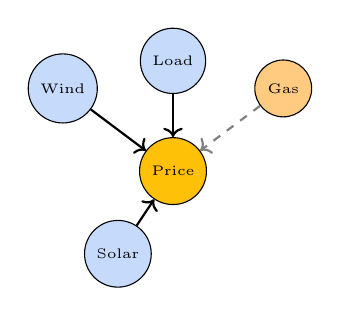
\begin{tikzpicture}[scale=0.7,
    node distance=1cm,
    var/.style={draw, circle, minimum size=0.6cm, font=\tiny}
]
\node[var, fill=elecyellow] (price) at (0,0) {Price};
\node[var, fill=causalblue!30] (wind) at (-2,1.5) {Wind};
\node[var, fill=causalblue!30] (load) at (0,2) {Load};
\node[var, fill=regimeorange!50] (gas) at (2,1.5) {Gas};
\node[var, fill=causalblue!30] (solar) at (-1,-1.5) {Solar};

\draw[->, thick] (wind) -- (price);
\draw[->, thick] (load) -- (price);
\draw[->, thick, dashed, gray] (gas) -- (price);
\draw[->, thick] (solar) -- (price);
\end{tikzpicture}
\end{center}
\textbf{Drivers:} Renewables + Load
\end{column}

\begin{column}{0.5\textwidth}
\textbf{Regime 1 (Crisis/High Volatility):}
\begin{center}
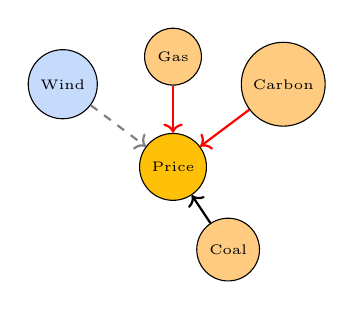
\begin{tikzpicture}[scale=0.7,
    node distance=1cm,
    var/.style={draw, circle, minimum size=0.6cm, font=\tiny}
]
\node[var, fill=elecyellow] (price) at (0,0) {Price};
\node[var, fill=causalblue!30] (wind) at (-2,1.5) {Wind};
\node[var, fill=regimeorange!50] (gas) at (0,2) {Gas};
\node[var, fill=regimeorange!50] (carbon) at (2,1.5) {Carbon};
\node[var, fill=regimeorange!50] (coal) at (1,-1.5) {Coal};

\draw[->, thick, dashed, gray] (wind) -- (price);
\draw[->, thick, red] (gas) -- (price);
\draw[->, thick, red] (carbon) -- (price);
\draw[->, thick] (coal) -- (price);
\end{tikzpicture}
\end{center}
\textbf{Drivers:} Fossil fuels + Carbon
\end{column}
\end{columns}

\vspace{0.2cm}
\begin{center}
\fcolorbox{lightgray}{white}{\parbox{0.9\textwidth}{
\textbf{Legend:} \quad
\tikz{\node[draw, circle, fill=elecyellow, minimum size=0.4cm] {};} Target (Price) \quad
\tikz{\node[draw, circle, fill=causalblue!30, minimum size=0.4cm] {};} Renewable/Load \quad
\tikz{\node[draw, circle, fill=regimeorange!50, minimum size=0.4cm] {};} Commodity (crisis driver)\\[0.1cm]
\quad 
\tikz{\draw[->, thick] (0,0) -- (0.5,0);} Strong causal \quad
\tikz{\draw[->, thick, red] (0,0) -- (0.5,0);} Crisis-dominant \quad
\tikz{\draw[->, thick, dashed, gray] (0,0) -- (0.5,0);} Weak/suppressed
}}
\end{center}
\end{frame}

\begin{frame}{What Drives Price Changes? Regime-Specific DAGs}
\textbf{Interpretation:}
\begin{itemize}
    \item \textbf{Normal regime:} Renewables (wind, solar) and load dominate price formation
    \item \textbf{Crisis regime:} Commodity prices (gas, carbon) become primary drivers
\end{itemize}
\end{frame}

%==============================================================================
\begin{frame}{How Does the Setting Matter?}
\begin{columns}
\begin{column}{0.5\textwidth}
\textbf{Task: Estimation vs Prediction}
\begin{itemize}
    \item \textbf{Estimation} ($Y_t | X_{0:t}, Y_{0:t-1}$):
    \begin{itemize}
        \item Higher accuracy (access to recent Y)
        \item Primarily autoregressive signal
        \item Univariate models excel
    \end{itemize}
    \item \textbf{Prediction} ($Y_{t+1} | X_{0:t}, Y_{0:t}$):
    \begin{itemize}
        \item More challenging
        \item Exogenous features more valuable
        \item Causal structure helps generalize
    \end{itemize}
\end{itemize}
\end{column}

\begin{column}{0.5\textwidth}
\textbf{Target: DE vs FR vs DE\_FR}
\begin{itemize}
    \item \textbf{FR}: Highly autoregressive
    \begin{itemize}
        \item DS3M\_UV achieves $\rho = 0.96$
        \item Nuclear baseload = stable dynamics
    \end{itemize}
    \item \textbf{DE}: More complex
    \begin{itemize}
        \item Higher renewable share
        \item More volatile, regime-dependent
    \end{itemize}
    \item \textbf{DE\_FR}: Joint modeling hardest
    \begin{itemize}
        \item Cross-country dependencies complex
        \item Information may interfere
    \end{itemize}
\end{itemize}
\end{column}
\end{columns}

\vspace{0.3cm}
\begin{center}
\textbf{Recommendation:} Use \textbf{DS3M\_UV} for FR, \textbf{CaRS} for DE when interpretability is needed
\end{center}
\end{frame}

%==============================================================================
\section{Outlook}

\begin{frame}{Future Work}
\begin{columns}
\begin{column}{0.5\textwidth}
\textbf{1. Seed Initialization Variance}
\begin{itemize}
    \item High variance across seeds ($\sigma > 0.1$)
    \item Is this causal or non-causal?
    \item \textbf{Solutions:}
    \begin{itemize}
        \item Better initialization schemes
        \item Ensemble methods
        \item Bayesian treatment of DAG parameters
    \end{itemize}
\end{itemize}

\vspace{0.3cm}
\textbf{2. Regime Collapse}
\begin{itemize}
    \item Often converges to 1 regime
    \item Need stronger regime regularization
    \item Entropy bonus for regime diversity
\end{itemize}
\end{column}

\begin{column}{0.5\textwidth}
\textbf{3. Additional Data Sources}
\begin{itemize}
    \item \textbf{TTF Gas}: European natural gas benchmark
    \item \textbf{API2 Coal}: Coal price index
    \item \textbf{EU ETS Carbon}: Carbon allowance prices
    \item Weather forecasts, demand forecasts
\end{itemize}

% \vspace{0.3cm}
\textbf{4. Model Enhancements}
\begin{itemize}
    \item \textbf{Ensembles:} Combine multiple seeds for robust predictions
    \item \textbf{Longer lags:} Currently lag=1, may benefit from lag=2+
    \item \textbf{Hierarchical DAGs:} Share common structure across regimes
\end{itemize}
\end{column}
\end{columns}
\end{frame}

\begin{frame}{Future Work}
\vspace{0.3cm}
\begin{center}
\fcolorbox{causalblue}{lightgray}{\parbox{0.9\textwidth}{\centering
\textbf{Key Challenge:} Balancing model complexity (more regimes, more edges)\\
with stability and interpretability.
}}
\end{center}
\end{frame}

%==============================================================================
\begin{frame}{Summary}
\begin{itemize}
    \item \textbf{CaRS} successfully combines regime switching (DS3M) with causal discovery (FANTOM)

    \item \textbf{Complete results:} All d=2,3,4 configurations now successful (80GB GPU resolved OOM issues)

    \item \textbf{Best results:}
    \begin{itemize}
        \item DE estimation d=2: $\rho = 0.74$; d=4: $\rho = 0.56$ (seed 123: $\rho = 0.84$)
        \item DE\_FR estimation d=3: $\rho = 0.47$ (seed 456: $\rho = 0.72$)
        \item Sparse DAGs: 3-6 high-confidence edges per regime
    \end{itemize}

    \item \textbf{Trade-offs:}
    \begin{itemize}
        \item DS3M\_UV better for pure autoregressive tasks (FR)
        \item CaRS better when interpretability needed (DE)
    \end{itemize}

    \item \textbf{Open challenges:} Regime collapse (esp. d=4), seed variance, cross-country modeling
\end{itemize}

\vspace{0.5cm}
\begin{center}
\Large\textbf{Questions?}
\end{center}
\end{frame}

%==============================================================================
%==============================================================================
\appendix
\section{Appendix}

%------------------------------------------------------------------------------
\begin{frame}{Appendix: Detailed Literature Review}
\textbf{Regime-Switching Models:}
\begin{itemize}
    \item Hamilton (1989): Markov-switching autoregressive models for business cycles
    \item Kim (1994): Dynamic linear models with regime switching
    \item Xu et al. (2021): \textbf{DS3M} -- Deep Switching State Space Model
\end{itemize}

\vspace{0.2cm}
\textbf{Causal Discovery Methods:}
\begin{itemize}
    \item Spirtes et al. (2000): PC algorithm for constraint-based discovery
    \item Chickering (2002): GES -- Greedy Equivalence Search
    \item Zheng et al. (2018): \textbf{NOTEARS} -- Differentiable DAG learning
    \item Ng et al. (2020): \textbf{GOLEM} -- Likelihood-based structure learning
    \item Pamfil et al. (2020): \textbf{DYNOTEARS} -- Time series extension
\end{itemize}

\vspace{0.2cm}
\textbf{Deep Causal Models:}
\begin{itemize}
    \item Geffner et al. (2022): \textbf{DECI} -- Deep End-to-end Causal Inference
    \item Gong et al. (2022): \textbf{Rhino} -- Historically dependent noise
    \item Rahmani et al. (2025): \textbf{FANTOM} -- Regime-switching causal discovery
\end{itemize}
\end{frame}

%------------------------------------------------------------------------------
\begin{frame}{Appendix: Literature Review (cont.)}
\textbf{Energy Price Modeling:}
\begin{itemize}
    \item Weron (2014): Electricity price forecasting -- comprehensive review
    \item Ziel \& Weron (2018): Day-ahead electricity price forecasting
    \item Lago et al. (2021): Deep learning for electricity price forecasting
    \item Marcjasz et al. (2023): Probabilistic electricity price forecasting
\end{itemize}

\vspace{0.3cm}
\textbf{State Space Models:}
\begin{itemize}
    \item Kalman (1960): Linear state estimation
    \item Durbin \& Koopman (2012): Time series analysis by state space methods
    \item Krishnan et al. (2017): Structured inference networks for nonlinear state space
    \item Rangapuram et al. (2018): Deep state space models for time series forecasting
\end{itemize}

\vspace{0.3cm}
\textbf{Variational Inference:}
\begin{itemize}
    \item Kingma \& Welling (2014): VAE -- Variational Auto-Encoders
    \item Rezende et al. (2014): Stochastic backpropagation
    \item Jang et al. (2017): Gumbel-Softmax for discrete latent variables
\end{itemize}
\end{frame}

%------------------------------------------------------------------------------
\begin{frame}{Appendix: Placeholder -- Regime Time Series Visualization}
\begin{center}
\fcolorbox{lightgray}{white}{\parbox{0.8\textwidth}{\centering
\vspace{2cm}
\textbf{[TO BE GENERATED]}\\[0.5cm]
Combined visualization showing:\\
(1) Price time series with regime coloring\\
(2) Regime probability curves\\
(3) Detected changepoints\\[0.5cm]
For DE, FR, and DE-FR markets
\vspace{2cm}
}}
\end{center}

{\scriptsize \textit{Figure will be generated from CaRS model runs on unified dataset.}}
\end{frame}

%------------------------------------------------------------------------------
\begin{frame}{Appendix: Placeholder -- Causal Feature Importance}
\begin{center}
\fcolorbox{lightgray}{white}{\parbox{0.8\textwidth}{\centering
\vspace{2cm}
\textbf{[TO BE GENERATED]}\\[0.5cm]
Bar chart showing:\\
Average edge weight magnitude $|W|$ per feature\\
Grouped by regime (side-by-side bars)\\
Separate panels for instantaneous vs. lagged effects\\[0.5cm]
Features: Wind, Solar, Gas, Coal, Load, Carbon, ...
\vspace{2cm}
}}
\end{center}

{\scriptsize \textit{Figure will be generated from CaRS sparsity sweep experiments with multiple lags.}}
\end{frame}

%------------------------------------------------------------------------------
\begin{frame}{Appendix: Placeholder -- Lag Analysis}
\begin{center}
\fcolorbox{lightgray}{white}{\parbox{0.8\textwidth}{\centering
\vspace{2cm}
\textbf{[TO BE GENERATED]}\\[0.5cm]
Comparison of model performance across lag settings:\\
lag=1, lag=2, lag=3, ...\\[0.5cm]
Metrics: Spearman $\rho$, Directional Accuracy, RMSE\\
Trade-off: more lags = more parameters but potentially better dynamics capture
\vspace{2cm}
}}
\end{center}

{\scriptsize \textit{Figure will be generated from CaRS experiments with varying lag configurations.}}
\end{frame}

\end{document}
